
%	Detector calibration

\section{Detector calibration}\label{Section_Calibration}
\Headerfooter{Detector calibration}
\vs\hs
In physics experiments, the data reliability can be obtained by performing the detector calibration precisely.
The detector calibration indicates comfirming if the detector is working properly and the measurement accuracy is sufficient.
If needed, it is also important to determine the parameters in MC to reproduce the experimental results.
The detector calibration in SK can be largely classified as follows.
\begin{itemize}
	\item ID detector calibration
	\item Photon tracking
	\item OD detector calibration
	\item Energy scale calibration
\end{itemize}
In this section, ID detector calibration, photon tracking, and energy scale calibration using the linear accerelator (LINAC) are described.
The OD detector calibration is described in Ref.~\cite{2014AbeCalib}.





\subsection{ID detector calibration}
\vs\hs
Before describing about each calibration, the procedure of ID detector calibration is described.
First, applied voltage of each ID PMT is determined to output the similar degree of charge in all ID PMTs.
This eliminates the asymmetry in the detector response and improves energy resolution.
Second, we understand the individual difference of gain and quantum efficiency (QE) of ID PMTs.
Here, gain is defined as the amplification factor of a photoelectron arrived to the PMT dinode.
%Also, QE is defined as the probability that a photon hitting the photocathode of a PMT is converted into a photoelectron.
Also, QE is generally defined as the probability that a photon hitting the photocathode of a PMT is converted into a photoelectron.
In SK, QE is defined also including the probability that a photoelectron arrives to the first dinode of a PMT.
Signals by high energy events like cosmic ray muons largely depends on gain.
While signals by low energy (DSNB and NCQE) events, which are mostly one photoelectron level, largely depends on QE.
Therefore, it is crucial to understand the gain and QE of each ID PMT since the reconstructed energy depends on the gain and QE.
Furthermore, the timing response of each ID PMT is calibrated to correct the deviation caused by the length of cables sending signals, the process time in electrical circuits, and the height of PMT signal waveforms.

\subsubsection{High-Voltage determiation}\label{Section_HV}
\vs\hs
Applied voltage of each PMT (High-Voltage, HV) is determined to output the similar degree of charge in all PMTs\footnote{In SK-V, HV was retuned so that the peak of charge distribution (see Figure~\ref{Calibration_Single-pe}) obtained by using Ni-Cf source (see Figure~\ref{Calibration_Ni}) match in all PMTs.}.
The HV determination is conducted by setting an isotropic light source (Xe light source) at the center of the SK tank.
The Xe light source consists of a Xe lamp, a UV filter, and a scintillation ball with a diameter of 5 cm.
Xe lamp emits light by applying voltage inside a glass tube filled with Xe gas.
Also, the scintillation ball includes 15 ppm\footnote{ppm stands for ``parts per million'', and 1 ppm is equal to 0.0001\%.} POPOP and 2,000 ppm magnesium oxide (MgO).
POPOP plays a role of converting the light wavelength, and MgO plays a role of emitting light from the scintillation ball as isotropically as posiible.\\
\hs
This measurement depends on not only the distance from the light source to a PMT, but also water transparency and photon reflectivity on the surface of PMTs.
To ensure accuracy, before this measurement, 420 pre-calibrated PMTs, termed standard PMTs, with individually determined HV were installed into the SK tank.
Figure~\ref{Calibration_CalibPMT} shows the location of standard PMTs in ID and schematic view of the grouping of nearby PMTs.
HV of a PMT other than standard PMTs is set so that the amount of charge obtained by the PMT matches the average amount of charge obtained by standard PMTs belonging to the PMT's group.
After determining the HV, the amount of charge was measured again by applying the determined HV to each PMT.
As a result, the difference between the amount of charge obtained by each PMT and the average value was within 1.3\% in RMS, which is consistent with the result of preliminary measurement for the standard PMTs.
Note that the Xe light source is installed to monitor the long-term gain fluctuations of PMTs even after the HV is determined.

\begin{figure}[h]
	\centering
	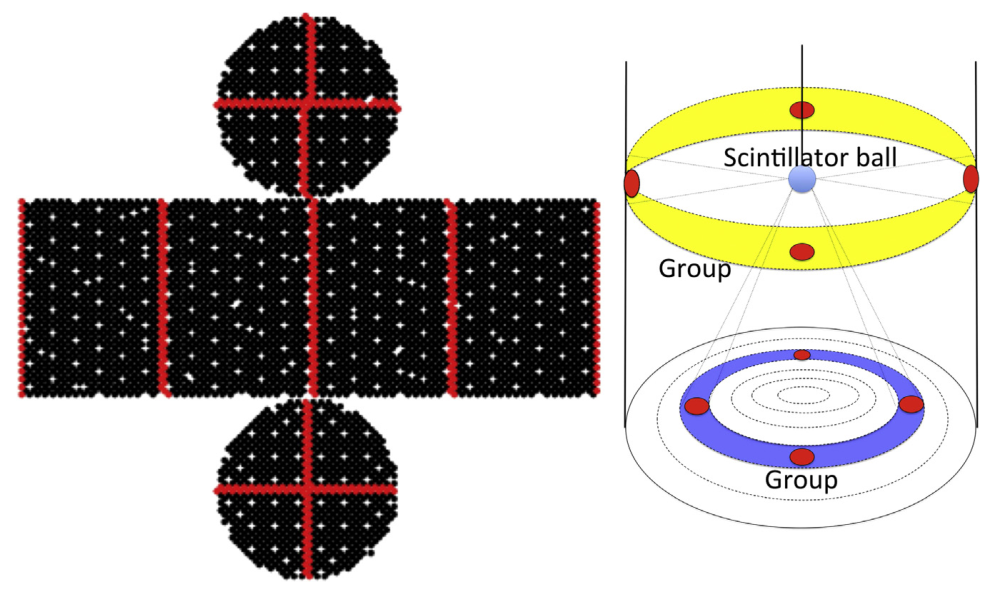
\includegraphics[width=10cm]{Figures/Calibration/CalibPMT}
	\caption[Location of standard PMTs in ID and schematic view of the grouping of nearby PMTs]{
	Location of standard PMTs in ID (left) and schematic view of the grouping of nearby PMTs (right)~\cite{2014AbeCalib}.
	Red points show standard PMTs. There are 17 groups on barrel, and 8 groups on top and bottom.
	}\label{Calibration_CalibPMT}
\end{figure}

\subsubsection{Relative gain measurement}
\vs\hs
To determine the gain of each PMT, we must understand the average gain of all PMTs (absolute gain) and the deviation from the average gain of all PMTs (relative gain).
To calculate this relative gain, we perform two-step measurements using an isotropic light source.
First, a high intensity light is applied so that all PMTs receive a sufficient amount of light.
We define the average value of the charge at the $i$-th PMT in this measurement as $Q_{\rm{obs}}(i)$.
Next, a low intensity light is applied so that PMTs receive only a small number of photons.
We define the number of hits (the number of recording the amount of charge exceeding a threshold) at the $i$-th PMT in this measurement as $N_{\rm{obs}}(i)$.
By performing these two measurements using the same light source and at the same position, $Q_{\rm{obs}}(i)$ and $N_{\rm{obs}}(i)$ can be calculated as
\begin{eqnarray}
	Q_{\rm{obs}}(i)&\propto&I_{\rm{H}} \times a(i) \times \epsilon(i) \times G(i),\label{Calibration_Eq_Q}\\
	N_{\rm{obs}}(i)&\propto&I_{\rm{L}} \times a(i) \times \epsilon(i),\label{Calibration_Eq_N}
\end{eqnarray}
where $I_{\rm{H}}$($I_{\rm{L}}$) shows the average amount of light of high (low) intensity, $a(i)$ shows the acceptance of the $i$-th PMT, $\epsilon(i)$ shows the QE of the $i$-th PMT, and $G(i)$ shows the gain of the $i$-th PMT.
By taking the ratio of Equation~(\ref{Calibration_Eq_Q}) and Equation~(\ref{Calibration_Eq_N}), $G(i)$ can be calculated as
\begin{eqnarray}
	G(i)\propto{Q_{\rm{obs}}(i) \over N_{\rm{obs}}(i)}.\label{Calibration_Eq_G}
\end{eqnarray}
Relative gain of each PMT can be obtained by normalizing Equation~(\ref{Calibration_Eq_G}) with the average gain of all PMTs.
Note that $I_{\rm{H}}/I_{\rm{L}}$ can also be ignored by this normalization.\\
\hs
As a result of this measurement, the RMS of the ralative gain distribution was found to be 5.9\%~\cite{2014AbeCalib}.
Since the HV of each PMT is set so that $Q_{\rm{obs}}(i)$ is the same among PMTs\footnote{As noted in the footnote of Section~\ref{Section_HV}, in SK-V, HV was retuned so that the peak of charge distribution (see Figure~\ref{Calibration_Single-pe}) obtained by using Ni-Cf source (see Figure~\ref{Calibration_Ni}) match in all PMTs.}, this difference is considered to be caused by the difference of QE for each PMT.
Relative gain of each PMT is used as the correction coefficient when converting the output charge into the number of photoelectrons.

\subsubsection{Absolute gain measurement}
\vs\hs
Absolute gain is used to convert the amount of charge recorded in pC to the number of photoelectrons (p.e.).
Absolute gain is determined from the charge distribution of 1 p.e. signals from a Ni-Cf source, which is a gamma-ray source.
Figure~\ref{Calibration_Ni} shows the picture of the Ni-Cf source.
The Ni-Cf source consists of a ball made from nickel oxide (NiO) and polyethylene, a brass rod, and $^{\text{252}}$Cf source.
$^{\text{252}}$Cf source emits neutrons through spontaneous fission, and the neutrons are thermalized while repeating elastic scattering with protons.
The thermalized neutron is captured on nickel nucleus, and gamma-rays are emitted isotropically.
When the Ni-Cf source is placed in the center of the SK tank, more than 99\% of signals are 1 p.e..

\begin{figure}[H]
	\centering
	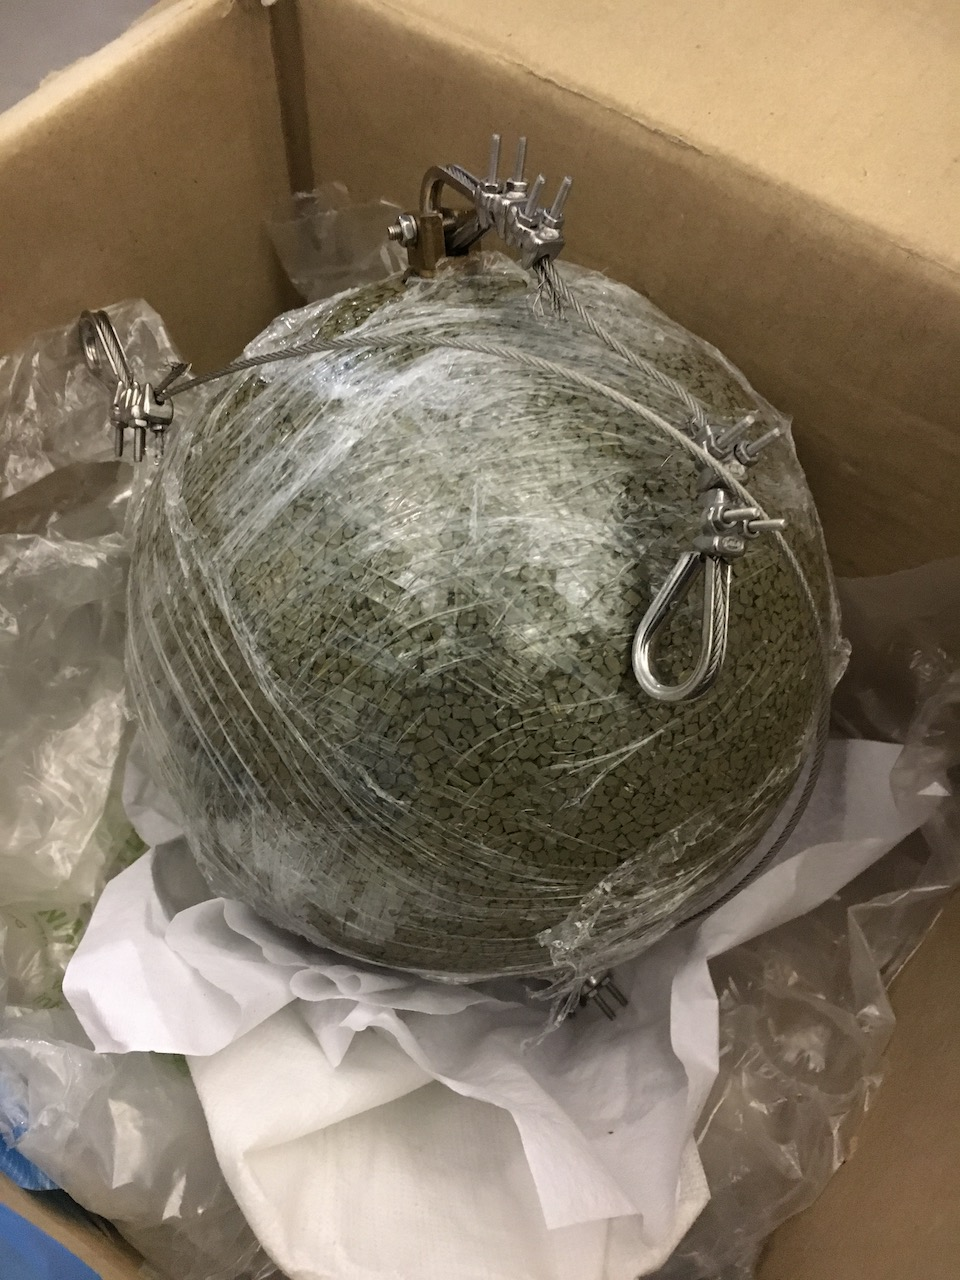
\includegraphics[width=6cm]{Figures/Calibration/Ni}
	\caption[Picture of the Ni-Cf source]{
	Picture of the Ni-Cf source.
	}\label{Calibration_Ni}
\end{figure}

\hs
Figure~\ref{Calibration_Single-pe} shows the charge distribution of the Ni-Cf source data in SK-III.
This distribution is obtained by applying the relative gain correction and adding up the charge distributions of all PMTs.
Also, to minimize the influence of PMT noise hits, the charge distributions are created at the time width that does not include signals due to the Ni-Cf source (off time) and the time width that includes signals due to the Ni-Cf source (on time), and the off time distribution is subtracted from the on time distribution.
Absolute gain is defined as the mean value over the full range of the distribution.
The values of absolute gain is 2.055, 2.297, 2.243, 2.645, 2.460 in SK-I to SK-V, respectively.
Absolute gain in SK-VI is the same as that in SK-V since HV is not changed from SK-V.

\begin{figure}[h]
	\centering
	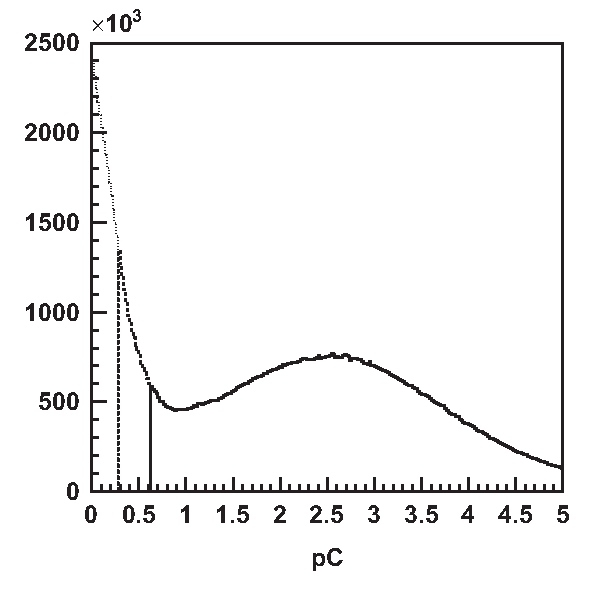
\includegraphics[width=8cm]{Figures/Calibration/Single-pe}
	\caption[Charge distribution of the Ni-Cf source data in SK-III]{
	Charge distribution of the Ni-Cf source data in SK-III~\cite{2014AbeCalib}.
	The dashed line shows the data with double gain and half threshold.
	The dotted line is linear extrapolation.
	}\label{Calibration_Single-pe}
\end{figure}

\subsubsection{Relative QE measurement}\label{Subsubsec_QE}
\vs\hs
Relative QE is also determined using the Ni-Cf source.
First, data is obtained by setting the Ni-Cf source at the center of the SK tank.
At that time, it is better to convect the ultrapure water so that the water quality is uniform.
Second, "hit rate" of each PMT ($R_{\rm Data}^{i}$) is calculated from the obtained data.
$R_{\rm Data}^{i}$ is defined as
\begin{eqnarray}
	R_{\rm Data}^{i} = {N_{\rm Hit}^{i} \times r_{i}^{2}/a(\theta_{i}) \over \displaystyle \sum^{N_{\rm PMT}} \{N_{\rm Hit}^{i} \times r_{i}^{2}/a(\theta_{i})\}/N_{\rm PMT}},
\end{eqnarray}
where $N_{\rm Hit}^{i}$ is the number of hits of $i$-th PMT, $r_{i}$ is the distance from the Ni-Cf source position to the position of $i$-th PMT, $a(\theta_{i})$ is the correction function of PMT acceptance, which is the same as Equation~(\ref{Recons_Eq_a_theta}), and $N_{\rm PMT}$ is the number of PMTs used in this calculation.
Finally, relative QE of each PMT ($QE_{i}$) is obtained by dividing $R_{\rm Data}^{i}$ by $R_{\rm MC}^{i}$, which is the hit rate of $i$-th PMT obtained from MC, to cancel the effects of reflection and water quality,
\begin{eqnarray}
	QE_{i} = {R_{\rm Data}^{i} \over R_{\rm MC}^{i}}.
\end{eqnarray}
Figure~\ref{Calibration_Hitrate} shows the hit rate distribution of data and MC.
In this figure, relative QE of each PMT is not considered in MC.
While, in data, the distribution is bumpy due to the effect of relative QE of each PMT.

\begin{figure}[h]
	\centering
	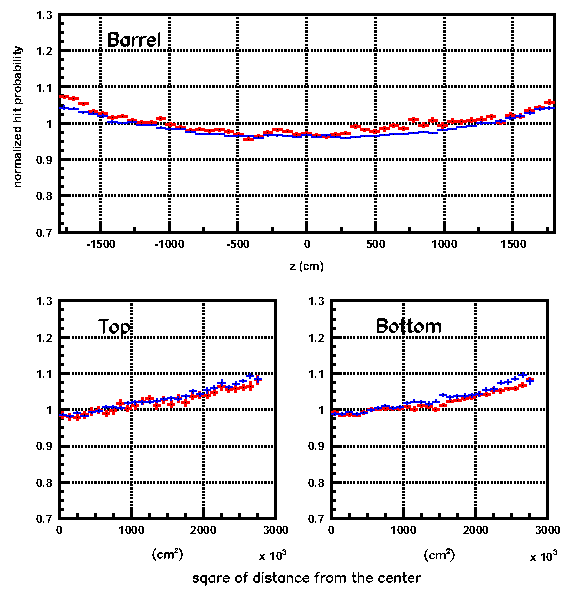
\includegraphics[width=12cm]{Figures/Calibration/Hitrate}
	\caption[Hit rate distribution of data and MC]{
	Hit rate distribution of data (red plots) and MC (blue plots)~\cite{2014AbeCalib}.
	Top, bottom left, and bottom right figure shows the distribution for barrel PMTs, top PMTs, and bottom PMTs, respectively.
	In the distribution for barrel PMTs, horizontal axis shows the z position of barrel PMTs.
	In the distributions for top and bottom PMTs, horizontal axis shows $x^{2} + y^{2}$, where $x$ and $y$ is the x and y position of top (bottom) PMTs, respectively.
	Vertical axis shows the average of $R_{\rm Data}^{i}$ or $R_{\rm MC}^{i}$ in each bin.
	}\label{Calibration_Hitrate}
\end{figure}

\subsubsection{Timing response calibration}
\vs\hs
The timing response of each PMT, which is important for reconstructing the trajectory and position of charged particles, deviates depending on the length of cables sending signals and the process time in electrical circuits.
Furthermore, the timing response depends on the height of PMT signal waveforms, which is known as the time walk effect.
The purpose of the timing response calibration experiment is to determine the correction factor of time walk for each PMT considering the process time of entire detector.\\
\hs
Figure~\ref{Calibration_TimingCalib} shows the schematic view of the timing response calibration system and cross section of the diffuser ball.
First, pulsed light with a wavelength of 337 nm and a full width at half maximum of 0.4 nsec is generated using a nitrogen laser.
The timing at which this pulsed light is generated is determined using a 2-inch PMT with a fast timing response.
After that, the wavelength of the pulsed light is shifted to 398 nm, where the QE of PMTs is high.
The pulsed light then goes through the optical fiber to the diffuser ball and is emitted isotropically.
Furthermore, the intensity of the pulsed light can be changed using an optical filter, and the timing response can be measured at various pulse heights.
Since the pulse height is proportional to the charge, this calibration is called TQ calibration.\\
\hs
In this measurement, as shown in Figure~\ref{Calibration_TQ}, a 2D distribution of timing and charge for one readout channel can be created.
This distribution is called a TQ map.
The timing information on the vertical axis in Figure~\ref{Calibration_TQ} is obtained by calculating the TOF (Time of Flight) from the positional relationship between the light source and the PMT and calculating T$\,-\,$TOF$\,-\,$T$_{\text{2-inch}}$, where T is the PMT hit timing and T$_{\text{2-inch}}$ is the signal transmission time of the 2-inch PMT.
A total of 15 correction factors can be obtained by fitting the peak at each QBin in the TQ map with the following polynomial function depending on QBin,
\begin{eqnarray}
	\text{QBin} \leq 10      &:& F_{1}(x) \equiv f_{3}(x), \\
	10 < \text{QBin} \leq 50 &:& F_{2}(x) \equiv F_{1}(10)+(x-10)\{F_{1}^{\prime}(10)+(x-10)f_{3}(x-10)\}, \\
	\text{QBin} > 50         &:& F_{3}(x) \equiv F_{2}(50)+(x-50)f_{6}(x-50), \\
	                         & & f_{N}(x) \equiv p_{0}+p_{1}x+p_{2}x^{2}+...+p_{N}x^{N},
\end{eqnarray}
where $F_{1}^{\prime}(x)$ is the derivative of $F_{1}(x)$.

\begin{figure}[H]
	\centering
	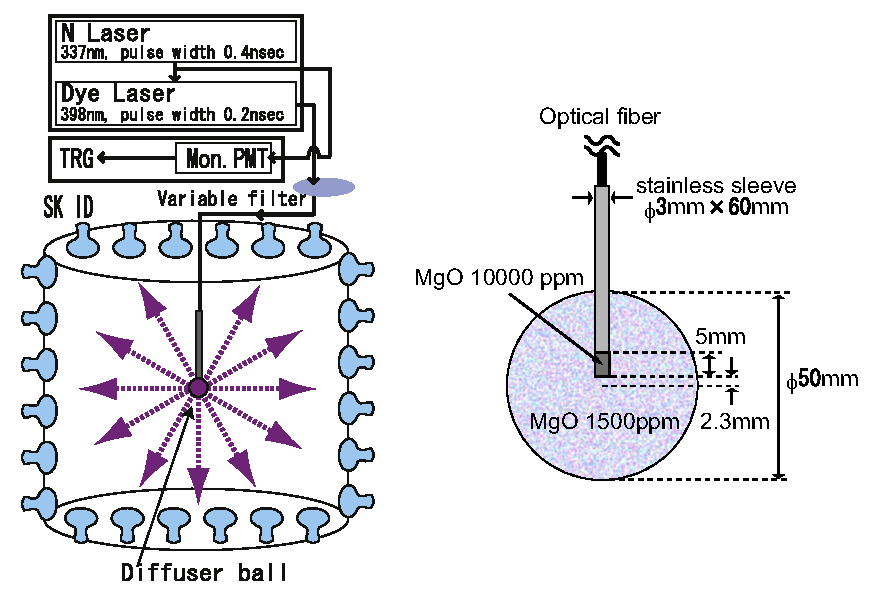
\includegraphics[width=10cm]{Figures/Calibration/TimingCalib}
	\caption[Schematic view of the timing response calibration system and cross section of the diffuser ball]{
	Schematic view of the timing response calibration system (left) and cross section of the diffuser ball (right)~\cite{2014AbeCalib}.
	}\label{Calibration_TimingCalib}
\end{figure}

\begin{figure}[H]
	\centering
	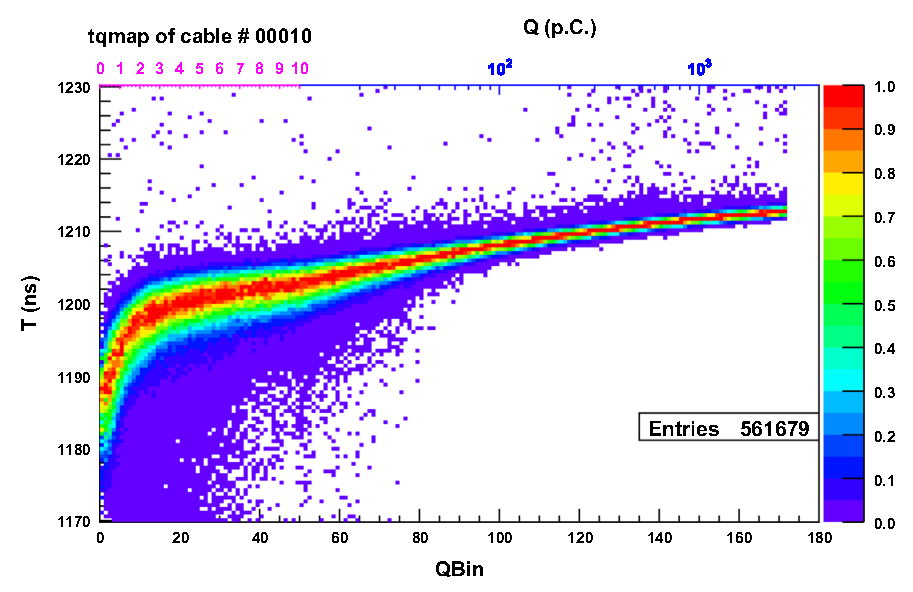
\includegraphics[width=12cm]{Figures/Calibration/TQ}
	\caption[2D distribution of timing and charge for one readout channel]{
	2D distribution of timing and charge for one readout channel~\cite{2014AbeCalib}.
	Horizontal axis shows charge (QBin) of each hit. Vertical axis shows TOF-corrected hit timing.
	}\label{Calibration_TQ}
\end{figure}





\subsection{Photon tracking}
\subsubsection{Water transparency measurement}\label{Subsubsec_Water}
\vs\hs
For photon tracking in MC, it is essential to consider the water properties like absorption and scattering.
The light attenuation is expressed as $\exp\{-l/L(\lambda)\}$, where $l$ is the light path length and $L(\lambda)$ is the attenuation length at wavelength $\lambda$.
Also, in MC, $L(\lambda)$ is defined as
\begin{eqnarray}
	L(\lambda)={1 \over \alpha_{\rm{abs}}(\lambda)+\alpha_{\rm{sym}}(\lambda)+\alpha_{\rm{asy}}(\lambda)},
\end{eqnarray}
where $\alpha_{\rm{abs}}(\lambda)$, $\alpha_{\rm{sym}}(\lambda)$, and $\alpha_{\rm{asy}}(\lambda)$ are attenuation coefficients of absorption, symmetric scattering, and asymmetric scattering at wavelength $\lambda$, respectively.
$\alpha_{\rm{sym}}(\lambda)$ is used to consider the Rayleigh scattering and the symmetric components of Mie scattering.
While $\alpha_{\rm{asy}}(\lambda)$ is used to consider the forward components of Mie scattering.\\
\hs
To determine each attenuation coefficient, laser light of various wavelengths (337, 375, 405, 445, and 473 nm) were applied downward from the top of the SK tank, and the PMT hit timing was measured.
Figure~\ref{Calibration_LaserCalib} shows the schematic view of the laser calibration system and TOF-subtracted hit timing distributions of the laser calibration data and MC.
Attenuation coefficients are determined using top PMTs that are 2 m away from the laser light injector, and barrel PMTs.
Barrel is separated into five regions, from B1 to B5.
B3 includes PMTs for 11 lines and the others include PMTs for 10 lines.
In the left side of Figure~\ref{Calibration_LaserCalib}, the cyan shaded circle spot on the bottom shows the beam target used for the TOF calculation.
Also, in the right side of Figure~\ref{Calibration_LaserCalib}, hits between the left two blue vertical solid lines are due to scattered photons, and this region is used to determine the attenuation coefficients.
The peaks in the right time region is thought to be due to photons reflected on the surface of PMT or black sheet.
Each attenuation coefficient is introduced into MC using the following formula based on experiments,
\begin{eqnarray}
	\alpha_{\rm{abs}}(\lambda) &=& P_{0} \times {P_{1} \over \lambda^{4}} + C, \\
	C                          &=& P_{0} \times P_{2} \times \biggl({\lambda \over 500}\biggr)^{P_{3}}, \\
	\alpha_{\rm{sym}}(\lambda) &=& {P_{4} \over \lambda^{4}} \times \biggl(1.0 + {P_{5} \over \lambda^{2}}\biggr), \\
	\alpha_{\rm{asy}}(\lambda) &=& P_{6} \times \biggl\{1.0 + {P_{7} \over \lambda^{4}} \times (\lambda - P_{8})^{2}\biggr\}.
\end{eqnarray}
Attenuation coefficients are determined so that $\chi^{2}$ is minimized by comparing the hit timing distribution of MC created while changing the nine parameters from $P_{0}$ to $P_{8}$ with the hit timing distribution of data.
Values of $P_{0}$ to $P_{8}$ are summarized in Table~\ref{tab:Calib_water_param}.

\begin{figure}[tbp]
	\centering
	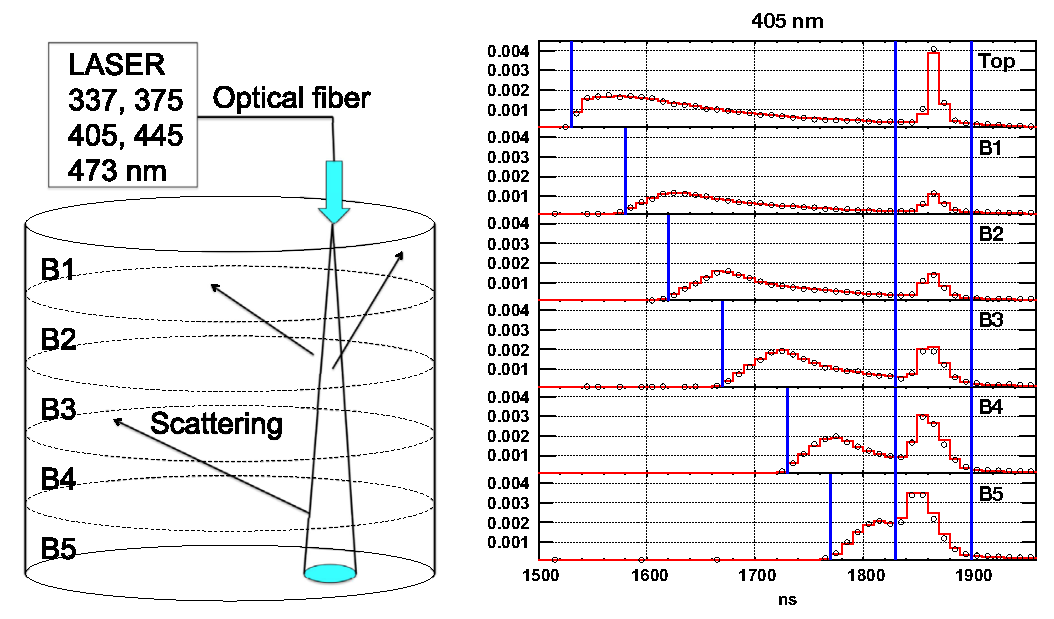
\includegraphics[width=12cm]{Figures/Calibration/LaserCalib}
	\caption[Schematic view of the laser calibration system and TOF-subtracted hit timing distributions of the laser calibration data and MC]{
	Schematic view of the laser calibration system (left) and TOF-subtracted hit timing distributions of the laser calibration data and MC (right)~\cite{2014AbeCalib}.
	Water parameter tuning is performed using top PMTs that are 2 m away from the laser light injector, and barrel PMTs.
	Barrel is separated into five regions, from B1 to B5.
	B3 includes PMTs for 11 lines and the others include PMTs for 10 lines.
	In the left figure, the cyan shaded circle spot on the bottom shows the beam target used in the TOF calculation.
	In the right figure, the black circle shows data and the red histogram shows MC.
	Both data and MC are normalized by observed total photoelectrons.
	Time region between the left two blue vertical solid lines is used for the water parameter tuning.
	Right time region is used for the PMT reflectivity measurement.
	}\label{Calibration_LaserCalib}
\end{figure}

\begin{table}[h]
	\centering
	\caption[Values of $P_{0}$ to $P_{8}$]{
	Values of $P_{0}$ to $P_{8}$.
	}\label{tab:Calib_water_param}
	\vs
	\begin{tabular}{cc} \hline \hline
		$P_{0}$ & $0.596600$               \\
		$P_{1}$ & $5.18888 \times 10^{7}$  \\
		$P_{2}$ & $1.06522$                \\
		$P_{3}$ & $14.1858$                \\
		$P_{4}$ & $1.13817 \times 10^{8}$  \\
		$P_{5}$ & $5.79108 \times 10^{4}$  \\
		$P_{6}$ & $2.26159 \times 10^{-4}$ \\
		$P_{7}$ & $17.1260$                \\
		$P_{8}$ & $4.48622 \times 10^{4}$  \\ \hline \hline
	\end{tabular}
\end{table}

\subsubsection{Top-Bottom Asymmetry}
\vs\hs
As described in Section~\ref{Section_WaterPuri}, the ultrapure water in SK is always circulated and purified by the water purification system.
The purified ultrapure water is supplied from the bottom of SK tank and collected at the top of SK tank.
The water quality gradually decreases as the ultrapure water moves from the bottom to the top of SK tank.
Therefore, the water transparency in the SK tank has position dependence, and it is crucial to understand the position dependence of water transparency precisely.
The vertical dependence is estimated by the Ni-Cf source data and the Xe light source data described in Section~\ref{Section_HV}.
The vertical asymmetry of water transparency (Top-Bottom Asymmetry, TBA) is defined as
\begin{eqnarray}
	{\rm TBA} = {N_{\rm top} - N_{\rm bottom} \over N_{\rm barrel}},
\end{eqnarray}
where $N_{\rm{barrel}}$, $N_{\rm{top}}$, and $N_{\rm{bottom}}$ shows the average number of ID PMT hits on the barrel, on the top, and on the bottom, respectively.
Figure~\ref{Calibration_TBA_SK56} shows the time variation of TBA in SK-V and SK-VI.
As described above, the water quality is better in the bottom side than in the top side.
Therefore, the values of TBA are negative.
Also, since the time variation seen in Figure~\ref{Calibration_TBA_SK56} are mainly due to the variation in absorption, the time and z-direction dependent water quality is implemented into the MC by multiplying $\alpha_{\rm{abs}}$ by the factor $A(z,t)$.
$A(z,t)$ is defined as
\begin{eqnarray}
	A(z,t) &\equiv& \left\{
	\begin{array}{ll}
		1 + z \times \beta(t) & (z\geq -11\,\rm{m}) \\
		1 - 11 \times \beta(t) & (z < -11\,\rm{m})
	\end{array} \right. , \\
		\beta(t) &=& -0.006322 \times 100 \times {\rm TBA} - 0.004130, \label{Calib_Eq_beta}
\end{eqnarray}
where $z$ is the z position and $\beta(t)\,[{\rm m}^{-1}]$ is the parameter indicating the degree of z dependence in water quality as a function of $t$.
In Equation~(\ref{Calib_Eq_beta}), ${\rm TBA}$ shows the TBA calculated by using the Xe light source data, and this equation can be obtained by using all Ni-Cf source data in SK-VI.

\begin{figure}[tbp]
	\centering
	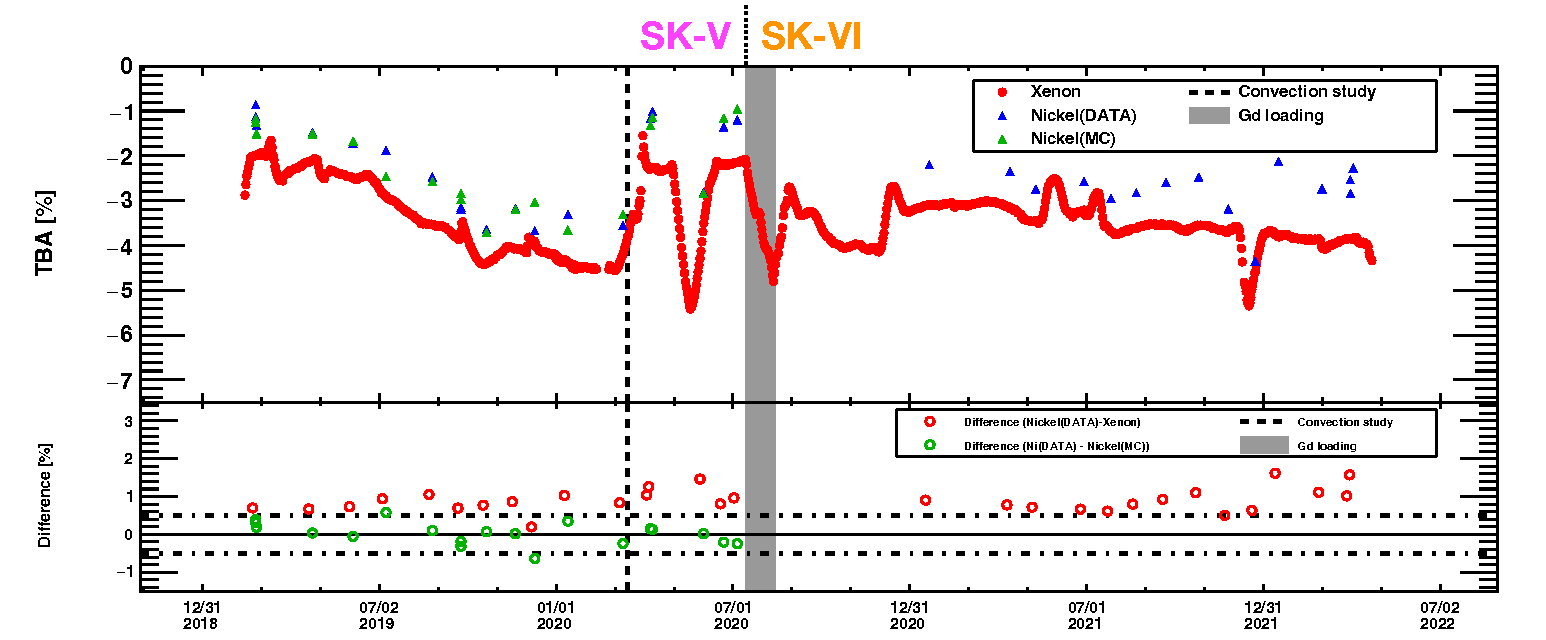
\includegraphics[width=16cm]{Figures/Calibration/TBA_SK56}
	\caption[Time variation of TBA in SK-V and SK-VI]{
	Time variation of TBA in SK-V and SK-VI~\cite{SK6LOWEdata}.
	The differences of TBA between Ni-Cf source data and Xe light source data and between Ni-Cf source data and MC are also shown on the bottom.
	The two thick horizontal dotted-dashed lines show the 0.5\% difference.
	}\label{Calibration_TBA_SK56}
\end{figure}

\subsubsection{Photon reflection on the material surface}
\vs\hs
When considering photon tracking, the photon reflection on the material surface must also be introduced into MC.
In this section, reflectivity measurements of PMT and black sheet are described.\\

\textbf{Reflection on the PMT surface}\\
\hs
The photon reflection on the PMT surface can be estimated by comparing the time region between the right two blue vertical solid lines in Figure~\ref{Calibration_LaserCalib} between data and MC.
The PMT surface consists of three layers of glass, bialkali, and vacuum.
In SK, the refractive indices of the glass, bialkali, and vacuum are defined as $1.472 + 3670/\lambda^{2}$, $n_{\rm re} + i \times n_{\rm im}$, and $1.0$, respectively.
Here, $\lambda\,[{\rm nm}]$ is the wavelength of a photon.
For bialkali, the complex refractive index is taken into account, where $n_{\rm re}$ and $n_{\rm im}$ are the real and imaginary parts of the complex refractive index, respectively.
The best value of $n_{\rm re}$ obtained by comparing the data with MC was 2.31 at $\lambda = 337\,{\rm nm}$, 2.69 at $\lambda = 365\,{\rm nm}$, 3.06 at $\lambda = 400\,{\rm nm}$, and 3.24 at $\lambda = 420\,{\rm nm}$.
While the best value of $n_{\rm im}$ obtained by comparing the data with MC was 1.667.\\

\textbf{Reflection on the black sheet surface}\\
\hs
Cherenkov photons are absorbed on the black sheet surface with high probability, but may also be reflected.
The black sheet reflectivity introduced into MC is adjusted by using the results of the measurement by laser injector.
Figure~\ref{Calibration_CalibBS} shows the schematic view of the black sheet reflectivity measurement.
First, laser injector is set at the center of the SK tank, laser light is injected onto a black sheet about 10~cm away, and the amount of charge by the reflected light ($Q_{\rm reflected}$) is measured.
Second, the amount of charge without black sheet ($Q_{\rm direct}$) is measured.
Finally, the black sheet reflectivity is adjusted by using the ratio $Q_{\rm reflected}/Q_{\rm direct}$.
As a result of adjusting the reflectivity, the difference between data and MC is within 1\%.
Note that this measurement was performed at three wavelengths (337~nm, 400~nm, 420~nm) and at three reflection angles ($30^{\circ}$, $45^{\circ}$, $60^{\circ}$).

\begin{figure}[H]
	\centering
	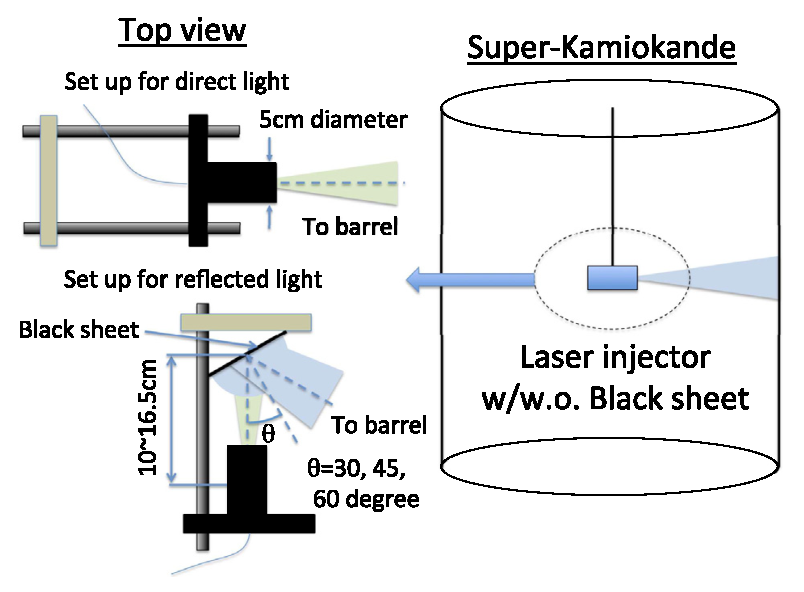
\includegraphics[width=10cm]{Figures/Calibration/CalibBS}
	\caption[Schematic view of the black sheet reflectivity measurement]{
	Schematic view of the black sheet reflectivity measurement~\cite{2014AbeCalib}.
	Left figure shows the top view.
	The laser light injector is inserted from the top center of the SK tank and the reflected light is measured by ID PMTs.
	}\label{Calibration_CalibBS}
\end{figure}





\subsection{LINAC}
\vs\hs
The energy scale parameter for low-energy MC simulations is determined by using the electron linear accelerator (LINAC)\footnote{The systematic uncertainty of energy scale is also determined by using LINAC.}.
Figure~\ref{Calibration_LINAC} shows the schematic view of LINAC~\cite{1999Nakahata}.
To suppress the effects of X-rays and gamma-rays emitted by LINAC itself, LINAC is set far from the SK detector.
Electron beams generated at LINAC are sent inside the detector with stainless beam pipes and magnets.
The kinetic energy of electron beams can be selected in the range of 5 to 18~MeV.
Moreover, the irradiate position of electron beams can be changed by extending and taking out the beam pipes.
In SK-VI, LINAC data was taken at three irradiate positions: ($-$1237, $-$70.7, 1197)~cm, ($-$1237, $-$70.7, $-$6)~cm, and ($-$1237, $-$70.7, $-$1209)~cm.
At each position, electron beams with kinetic energies of 8~MeV, 12~MeV, and 15~MeV were irradiated.
As for the position of ($-$1237, $-$70.7, $-$6)~cm, electron beams with kinetic energy of 6~MeV were also irradiated.
The energy scale parameter is derived by comparing $N_{\rm eff}$ between LINAC data and LINAC MC.
In SK-VI, the parameter was determined to be about 0.88, and this parameter is multiplied by QE of ID PMTs in MC simulations.

\begin{figure}[tbp]
	\centering
	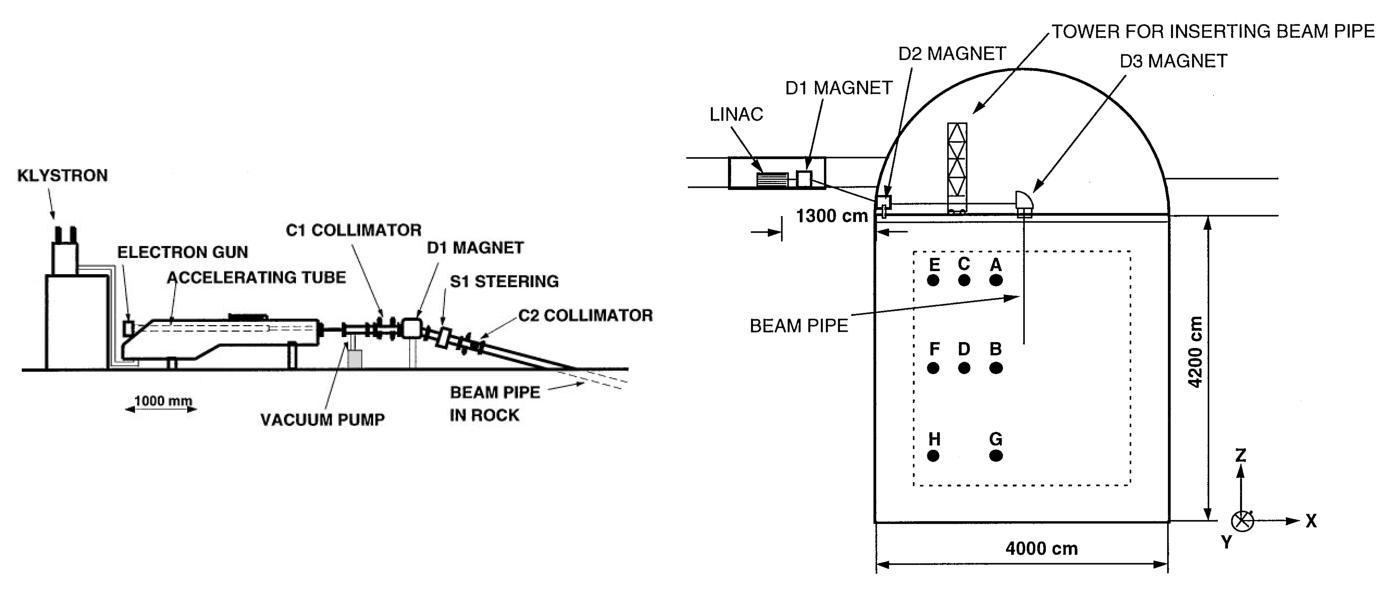
\includegraphics[width=16cm]{Figures/Calibration/LINAC}
	\caption[Schematic view of LINAC]{
	Schematic view of LINAC~\cite{1999Nakahata}.
	}\label{Calibration_LINAC}
\end{figure}





\newpage

